\title{Computer Vision}
\author{
        Assignment 4 - Retargeting\\
Spring 2023
}
\date{}
\documentclass[12pt]{article}
\usepackage[margin=0.7in]{geometry}
\usepackage{graphicx}
\usepackage{float}
\usepackage{amsmath}


\begin{document}
\maketitle


\section*{Introduction}
For this assignment we are going to implement some image retargeting approaches, allowing us to change the size and aspect ratio of an image.   Techniques will include sub-sampling and seam carving. 



\section*{Grading}
\begin{table}[h]
\begin{centering}
\begin{tabular}{|l|l|}
\hline
Theory Questions & 35pts \\
Image Resizing & 15pts\\
Energy Matrix & 10pts \\
Optimal Seam Discovery & 20pts\\
Seam Removal & 20pts\\
\hline
\textbf{TOTAL} & 100pts\\
\hline
\end{tabular}
\caption{Grading Rubric}
\end{centering}
\end{table}

\newpage
\section{(35pts) Theory Questions}
\begin{enumerate}
\item Given the grayscale image, $I$, below, if the top left location in our image is $(x=1,y=1)$, what would be value of a pixel at location $x=2.7, y=3.1$, if we were to:
	\begin{enumerate}
	\item Use the nearest neighbor in $I$. (3pts)
	\item Perform bi-linear interpolation using $I$.  Show your supporting work. (7pts)
	\end{enumerate}

$$
I=\begin{bmatrix}
2&	3&	4&	5&	1\\
1&	0&	2&	2&	1\\
4&	3&	5&	1&	2\\
4&	4&	4&	4&	6\\
4&	5&	2&	0&	2\\
2&	3&	3&	0&	3\\
\end{bmatrix}
$$	

\item If the matrix below is the gradient magnitude image
$$G =
\begin{bmatrix}
2&	3&	4&	5&	1\\
1&	0&	2&	2&	1\\
4&	3&	5&	1&	2\\
4&	4&	4&	4&	6\\
4&	5&	2&	0&	2\\
2&	3&	3&	0&	3\\
\end{bmatrix}
$$

\begin{enumerate}
\item Construct the cost matrix if we assume vertical seams (10pts).
\item What is the optimal seam (2pts)?
\end{enumerate}

\newpage
\item In lecture we discussed applying Poisson Blending to a simple 1D case.  Now let's extend this for the 2D case (after all, we're dealing with images!)!.

For simplicity, let's assume a $1\times1$ square mask.  Figure \ref{masks} shows two images, the one we're copying \emph{to} and the one that we're copying \emph{from}.  The masked area is indicated in green.

\begin{figure}[H]
\begin{center}
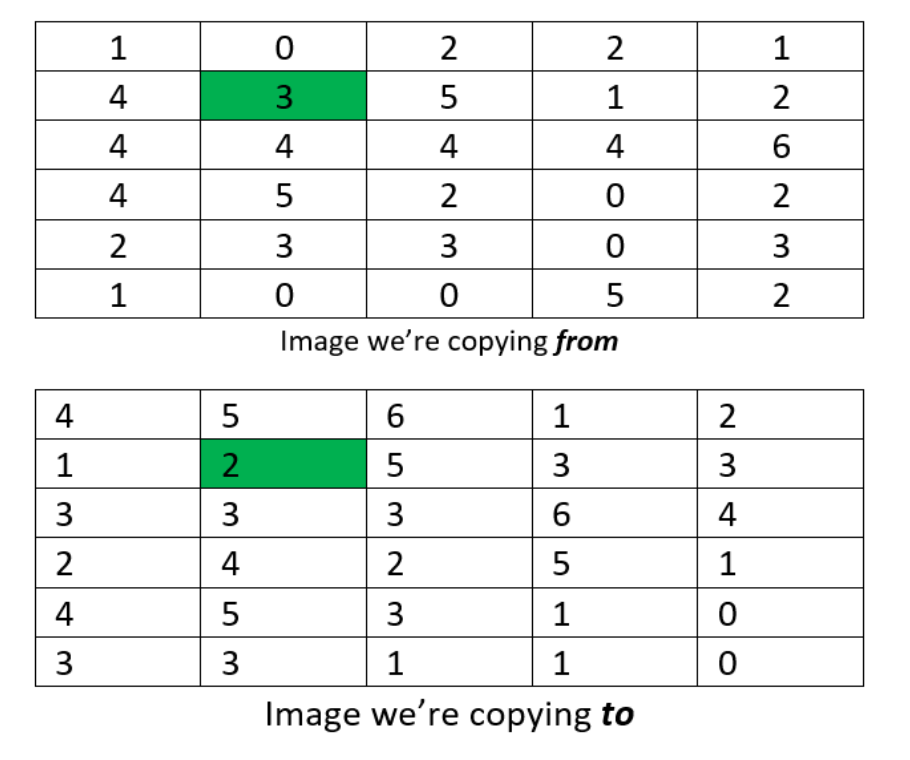
\includegraphics{masks.png}
\caption{Images for Theory Question \#3}
\label{masks}
\end{center}
\end{figure}

\begin{enumerate}
\item (5pts) First let's establish the cost function $J$ for this 2D case.  We'll once again use the squared error.  To avoid confusion between the unknowns $x$ and the direction $x$, we'll use $t$ for the values in our \emph{target} image (as opposed to $x$ in the 1D example).\\

\noindent
The cost with regards to pixel $(i,j)$ and the \emph{x-gradient} is as follows.  It's basically the same as the 1D case in the lecture slides:
$$J_{i,j}^x = ((t_{i,j} - t_{i-1,j})  - (s_{i,j} - s_{i-1,j}))^2$$

The cost for this same pixel, with regards to the \emph{y-gradient} is:
$$J_{i,j}^y = ((t_{i,j} - t_{i,j-1}) - (s_{i,j} - s_{i,j-1}))^2$$

Write out the terms of $J^x_{i,j}$ and $J^y_{i,j}$ that include at least one unknown in the target image.\\

\item (5pts) Using your answer from the previous part, what is the coeficient matrix $A$, the unknown vector $t$ and the known vector $b$ so that we can write $J$ as $J=(At-b)^T(At-b)$?  You should have a single matrix $A$ and a single vector $b$.\\

\item (3pts)  Finally, what are the values for the new pixel within the target mask?  For partial credit, make sure it's clear where you got your values from.\\
\end{enumerate}
\end{enumerate}


\newpage
\section{(15 points) Image Resizing}
First grab two images of interest to you so that we can multiple example I/O of each approach.   Next allow a user (either via prompt, parameter passing, or changing variable values) to provide a desired height and width.\\ 

\noindent
We'll refer to the original height and width as $h$ and $w$, respectively, and the new height and width as $h^{\prime}$ and $w^{\prime}$, respectively.  Do this all in color!  You may \textbf{not} use any Matlab functions (for instance, \emph{imresize} or \emph{interp2}) to do these changes for you.\\   

\noindent
Implement the following resizing techniques:
\begin{itemize}
\item Do nearest neighbor sampling.   Go through each location in your new target image, $(x^{\prime}, y^{\prime})$, and assign it the value of the nearest pixel, whose location is $(x, y) = round(x^{\prime} \frac{w}{w^{\prime}}, y^{\prime} \frac{h}{h^{\prime}})$.
\item Do bi-linear interpolation.   Go through each location in your new target image, $(x^{\prime}, y^{\prime})$, and compute the \emph{ideal} floating point location as $(x, y) =(x^{\prime} \frac{w}{w^{\prime}}, y^{\prime} \frac{h}{h^{\prime}})$.  Compute the values for location $(x^{\prime}, y^{\prime})$ by linearly interpolating the values of the four pixels nearest $(x,y)$.
\end{itemize}

\noindent
For your report provide sample I/O for both your test images, using both of these techniques, for two different values of $(w^{\prime}, h^{\prime})$ (8 total images).
\newpage

\section{(10 points) Energy Function}
We're also going to want to explore seam carving.  The first part of that requires computing the energy functions of your images.\\

\noindent
For each of your images, compute its energy and visualize this as an image.\\

\noindent
Some implementation details:
\begin{itemize}
\item Do this in grayscale
\item First smooth your grayscale image using a Guassian filter prior to getting the gradients (or do this in one step).  Choose parameters that make sense for you (and report them!).
\end{itemize}

\noindent
Since you already demonstrated in prior assignments your to implement RGB to Gray, Gaussian and Gradient kernels and convolution, for this assignment \textbf{may} use Matlab functions like $conv2, rgb2gray$.
\noindent
An example can be found in Figure \ref{fig1}

\begin{figure}[H]
\begin{center}
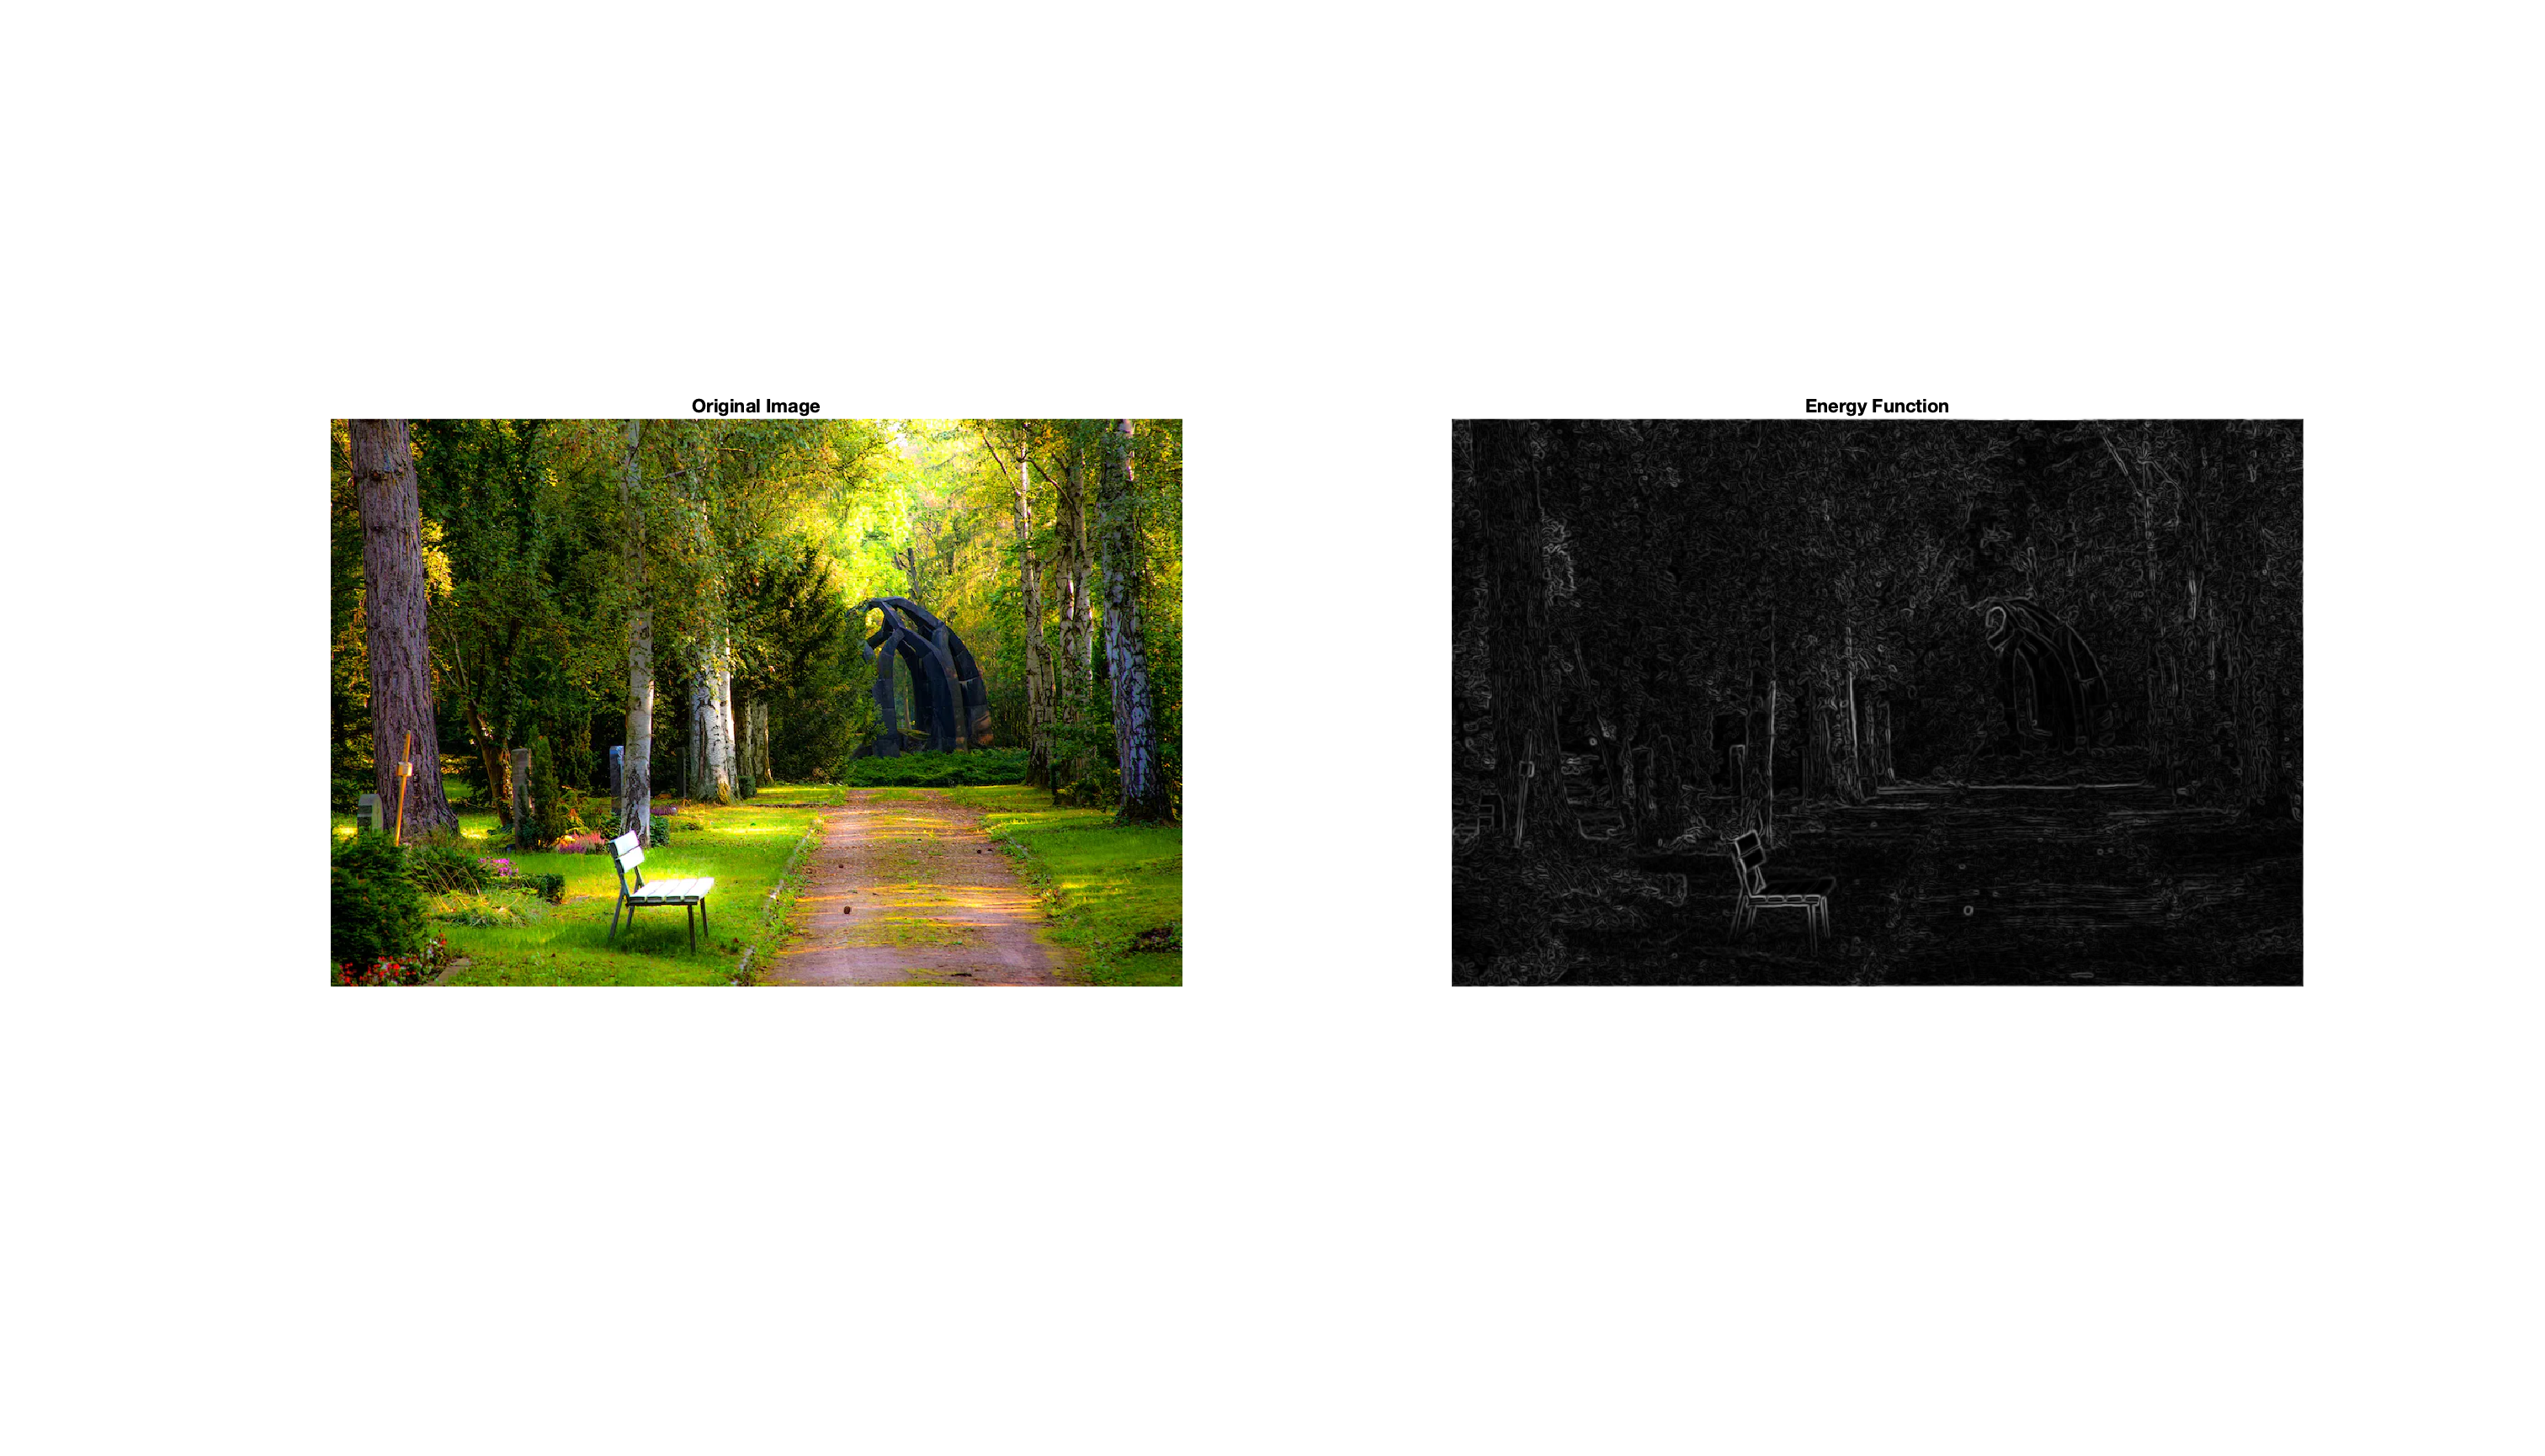
\includegraphics{energy.png}
\caption{Image Energy}
\label{fig1}
\end{center}
\end{figure}

\newpage

\section{(20 points) Optimal Seam}
Now that you have your energy images, we must find the optimal seam in it.\\

\noindent
Using the technique discussed in class, for each of your images, 

\begin{itemize}
\item Use its energy image to compute a seam matrix.
\item Find the optimal seam in this seam matrix via backtracing.
\item Superimpose on your color image the optimal seam in red.
\end{itemize}

\noindent
Additional Details:
\begin{itemize}
\item We will do vertical seam carving, starting at the top of the image.
\item You’ll likely have to think about how to handle the edge cases.
\end{itemize}

\noindent
Figure \ref{fig2} shows an example output.

\begin{figure}[H]
\begin{center}
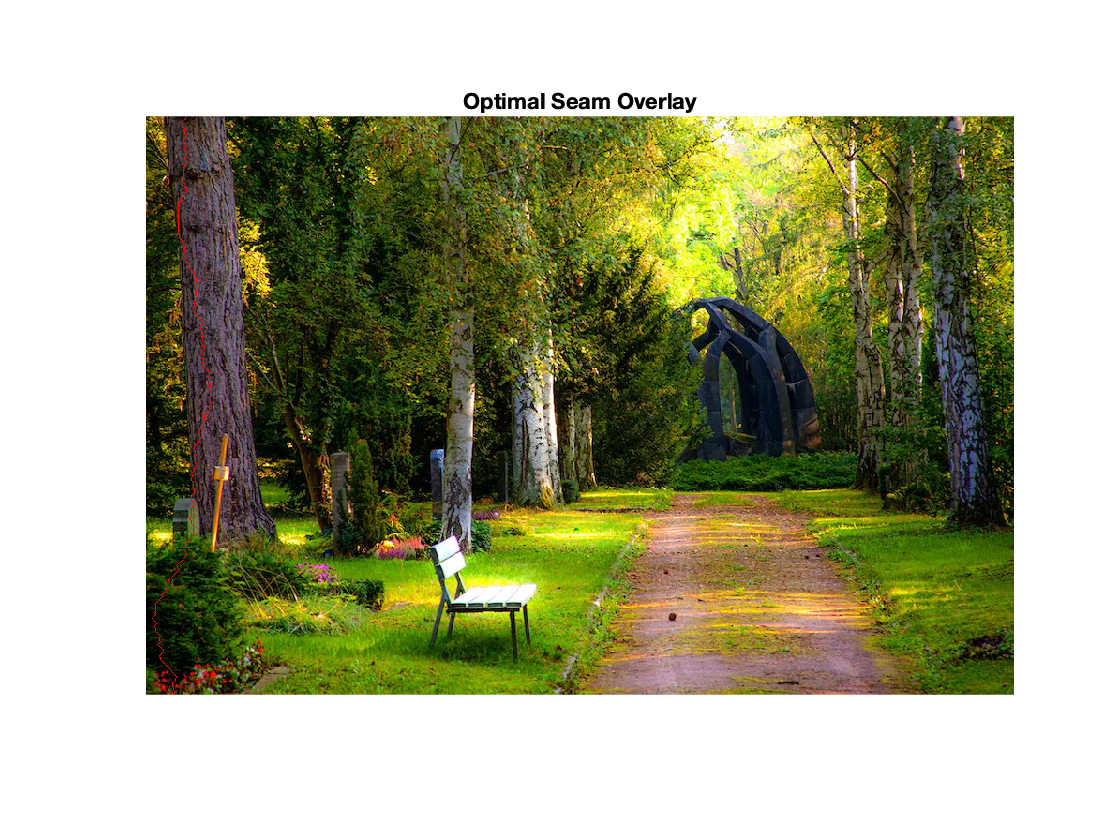
\includegraphics{seam.png}
\caption{Optimal Seam}
\label{fig2}
\end{center}
\end{figure}

\newpage

\section{(20 points) Seam Carving}
Finally, let's use seam carving to reduce the aspect ratio. Since we found the optimal \emph{vertical} seam in the previous part, we'll just reduce the width, from it's original width down to one pixel wide. \\

\noindent
For each of your images, create a video showing the seam removal process.  Each frame of the video should depict the current color image with the current optimal seam superimposed (like in the previous part). \\

\noindent
Note:
\begin{itemize}
\item You may need to “pad” your frames so that they all have the same size in order to render as a movie.
\item To create a movie in Matlab use the \emph{VideoWriter} class.  In addition, to keep the movies relatively small in file size, use the \emph{MPEG-4} profile for your VideoWriter object.
\end{itemize}

\newpage
\section*{Submission}
For your submission, upload to Blackboard a single zip file containing:

\begin{enumerate}
\item PDF writeup that includes:
\begin{enumerate}
\item Your answer to the theory question(s).
\item Your two original images.
\item Eight resized images for Part 2
\item Your two energy function images for Part 3.
\item Your two optimal seam images for Part 4.
\end{enumerate}
\item A README text file (not Word or PDF) that explains
\begin{itemize}
\item Features of your program
\item Name of your entry-point script
\item Any useful instructions to run your script.
\end{itemize}
\item Your source files
\item The chosen images that you are processing.
\item The videos generated for Part 5.
\end{enumerate}
\end{document}

